\documentclass[a4paper,12pt,titlepage]{article}
\usepackage[T1]{fontenc}
\usepackage[portuguese]{babel}
\usepackage[utf8x]{inputenc}
\usepackage{indentfirst}
\usepackage{graphicx}
\usepackage{times}
\usepackage{ucs}
\usepackage{float}    
\usepackage{fancyvrb}   
\usepackage{verbatim}
\usepackage{listings}
\usepackage{xcolor}
\usepackage{caption}
\usepackage{hyperref}
\usepackage{epigraph}
\captionsetup[figure]{width=10cm, font=small}

\DeclareCaptionFont{white}{\color{white}}
\DeclareCaptionFormat{listing}{%
  \parbox{\textwidth}{\colorbox{gray}{\parbox{\textwidth}{#1#2#3}}\vskip-4pt}}
\captionsetup[lstlisting]{format=listing,labelfont=white,textfont=white}
\lstset{frame=lrb,xleftmargin=\fboxsep,xrightmargin=-\fboxsep,language=[LaTeX]{TeX},columns=flexible}
\renewcommand{\lstlistingname}{Código}
\lstloadlanguages{Ruby}
\lstset{%
  basicstyle=\ttfamily\color{black},
  commentstyle = \ttfamily\color{red},
  keywordstyle=\ttfamily\color{blue},
  stringstyle=\color{orange}}

\hyphenation {pro-gra-ma pro-gra-mas com-pu-ta-cio-nais e-exem-plo pro-ble-mas
i-deia e-xer-c\'{i}-cios-pro-gra-mas e-xer-c\'{i}-cio-pro-gra-ma} 

\hypersetup{
    colorlinks=true, 
    linkcolor=black, 
    citecolor=black, 
    filecolor=black, 
    urlcolor=blue 
}

\title{Trabalho de Conclusão de Curso \\
Physimulation - Animação de Fenômenos Físicos}

\author{Rafael Issao Miyagawa \and Alberto Hideki Ueda \and
	{\small rafael.miyagawa@usp.br \ \ \ \ \ \ \ } \and {\small alberto.ueda@usp.br} \\ \ \and    
	Orientadores: José Coelho de Pina Junior \and  João Pedro Kerr Catunda }
\date{Novembro de 2012}

\begin{document}
\maketitle

\vspace*{\fill}
\epigraph{\it The most exciting phrase to hear in science, the one that heralds new discoveries, is not 'Eureka!' but 'That's funny ...'}{Isaac Asimov}
\newpage

\tableofcontents
\pagebreak

\part{Parte objetiva}
\section{Introdução} \label{introducao}

O foco deste projeto é atrair a atenção dos alunos do IME em relação a disciplina de física ministrada no curso de bacharelado em ciência da computação.
Com o simulador podemos integrar melhor os alunos aos assuntos abordados na física com demonstrações de ambientes físicos, 
integrando exercícios programas (EP) e também para ser utilizado em sala de aula.

\subsection{Física na computação}

A disciplina de Física (FAP-0126), oferecida no curso de BCC, é puramente teórica e não mostra nenhuma relação com a Ciência da Computação. Isso torna a disciplina menos interessante e frequentemente faz os alunos pensarem: "Para que serve esta disciplina?".
Para motivar os alunos e ilustrar melhor a relação entre as disciplinas básicas (Física, Estatística, Álgebra e Cálculo) com a Ciência da Computação, pretendemos criar uma biblioteca gráfica de simulação. Esta biblioteca será capaz de realizar uma leitura de dados de uma simulação de um EP e mostrar graficamente o resultado da simulação, por exemplo.
Esta biblioteca também proporcionará um ambiente de simulação específico e pronto para ser mostrado em salas de aula.
\subsection{Integração com a computação}

Existem muitos problemas ao tentar simular um ambiente físico com a computação. Temos o problema do tempo de simulação, 
que é o tempo que damos para os objetos físicos se interagirem e tomar o rumo necessário para refletir a realidade.
Existem alguns conceitos como broad phase, que é a fase em que os objetos são filtrados para realizarmos depois a narrow phase que é onde verificamos se aconteceu 
alguma colisão entre os objetos.

\subsection{Simulador}

A idéia do simulador é poder mostrar os problemas que encontramos ao tentar simular um ambiente físico com montagem de demonstrações. 

\newpage

\section{Plataforma computacional} \label{plataforma}
\subsection{Esquema de dependências}
O Physimulation depende de três bibliotecas: Chipmunk, Gosu e Glade. O programa começa com a leitura de dados com a interface criada com o Glade. Após a leitura, 
os dados lidos são convertidos em informações para que o Chipmunk possa processar e devolver o resultado da simulação. Os resultados das simulações são animadas 
com o Gosu. Toda interação entre as bibliotecas é feito com a linguagem Ruby.

A figura 1 representa um resumo do esquema de dependências entre as bibliotecas e o fluxo da dados da simulação.

\begin{figure}[!htbp]
  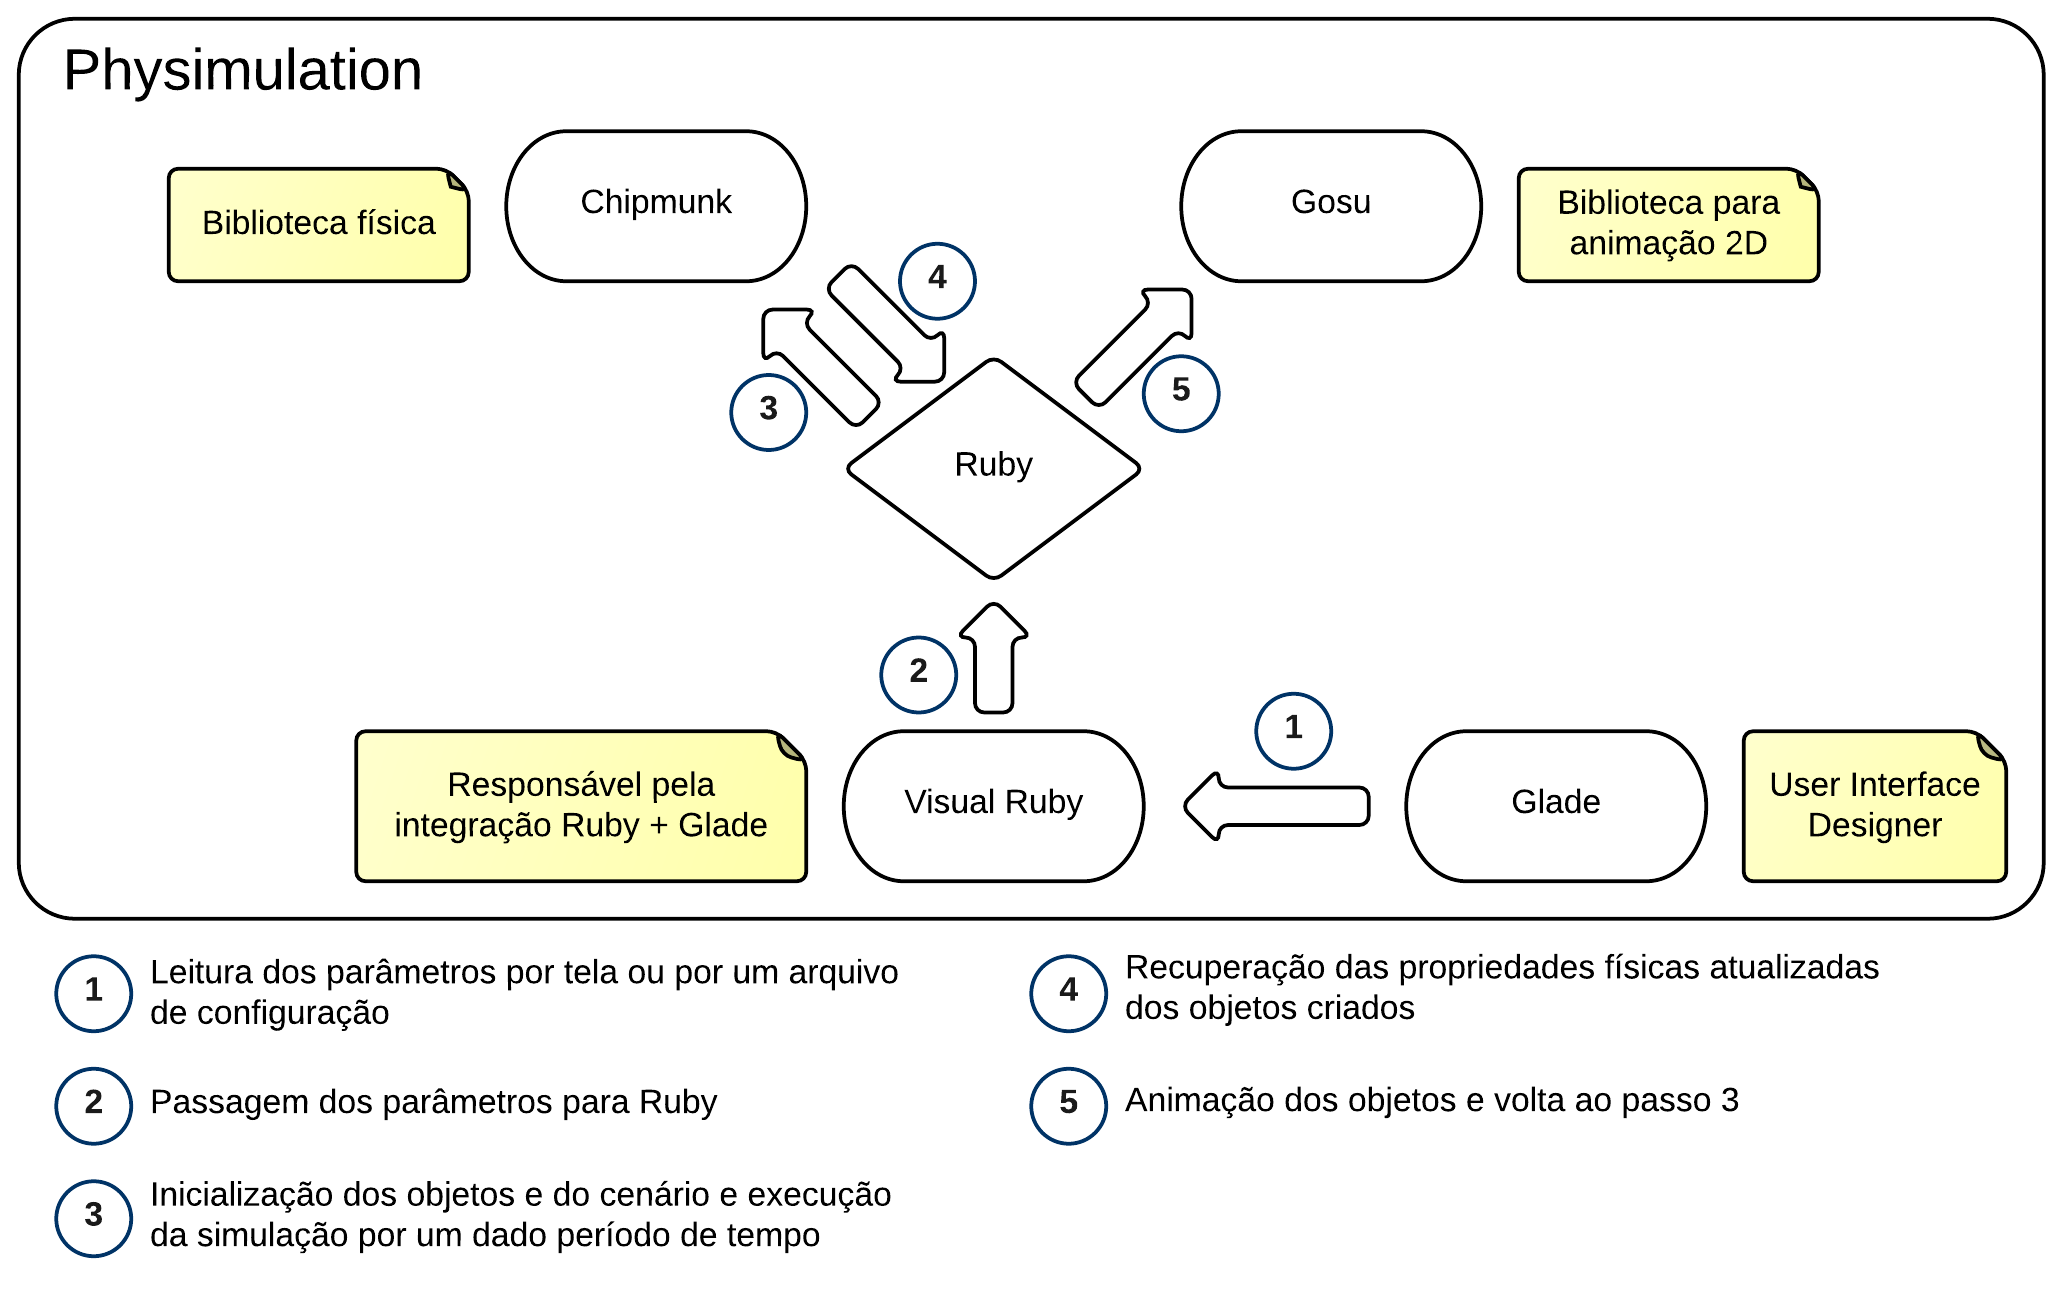
\includegraphics[scale=0.2]{EsquemaDependencia.png}
  \caption{Esquema de dependências do Physimulation}
\end{figure}

Nas seções seguintes mostraremos algumas características das ferramentas utilizadas no Physimulation.

\subsection{Ruby}
É a linguagem de programação utilizada no Physimulation para integrar todas as bibliotecas.
Ruby é puramente orientado a objetos, ou seja, tudo é objeto em ruby. O Código 1 apresenta um exemplo de um método dos números, criado no Physimulation, onde o 
número é convertido de radianos para grau:

\begin{lstlisting}[language=Ruby, caption=Conversão de radianos em graus]
  def graus = 3.14.radians_to_degrees
\end{lstlisting}

Ruby também permite ao programador alterar partes da própria linguagem, tornado-a flexível. Podemos alterar comportamentos de classes ou objetos 
em tempo de execução. Um exemplo é listado no Código 2, onde adicionamos o método radians\_to\_degrees na classe Numeric: 

\begin{lstlisting}[language=Ruby, caption=physics.rb ]
class Numeric
 def radians_to_degrees
    self * 180 / Math::PI
    end
 end
\end{lstlisting}

Outro recurso interessante utilizado no Physimulation são blocos. Os Blocos podem ser anexados a qualquer método descrevendo como deve ser 
o comportamento da execução deste método. O Código 3 mostra um exemplo do uso de blocos em Ruby. Neste exemplo, passamos um bloco ao método velocity\_func 
par atualizar a velocidade do objeto em relação a força gravitacional da lua e da terra: 

\begin{lstlisting}[language=Ruby, caption=RocketSimulation.rb]
    self.body.velocity_func { 
      |body, gravity, damping, dt|

      @earth_a = get_earth_acceleration(self)
      @moont_a = get_moon_acceleration(self)

      def self_a = vec2(@earth_a + @moon_a, 0)

      self.body.update_velocity(self_a, damping, dt)
    }
\end{lstlisting}

\subsection{Simulação com Chipmunk}
Chipmunk é uma biblioteca física 2D escrita em C que permite criar objetos convexos e segmentos que se interagem em um ambiente físico. Para criar os 
objetos para simulação é preciso definir as propriedades físicas e a forma do objeto. Após a criação precisamos adicioná-la à um ambiente físico para podermos 
iniciar a simulação.

Para criar o objeto é necessário primeiro definir o corpo. O corpo do objeto pode ser estático ou não. Um corpo estático é o corpo que não precisa de
massa e momento de inércia pois não é influenciado por nenhuma força física, se mantendo fixo no ambiente. Código 4 mostra como criar o corpo de um objeto:

\begin{lstlisting}[language=Ruby, caption=physics.rb]
  if options[:static]
    @body = CP::StaticBody.new
  else
    @body = CP::Body.new(massa, momento_inercia)
    @body.v = velocidade
    @body.w = velocidade_angular
  end

  @body.p = vetor_posicao
  @body.a = angulo
\end{lstlisting} 

Após a definição das propriedades físicas de um objeto, é necessário definir a forma do objeto para o Chipmunk tratar as colisões. No Chipmunk é 
possível criar três formas primitivas: Segmentos, círculos e polígonos convexos. No Physimulation criamos as formas de acordo com os parâmetros enviados
pela tela inicial. É necessário passar o corpo associado a forma no momento da criação. O código 5 mostra como são criados as formas no Physimulation:

\begin{lstlisting}[language=Ruby, caption=physics.rb]
  def self.factory(body, params = {})
    # Se existe um raio, criamos um circulo
    if params.has_key? :radius
      return Shape::Circle.new(body, 
        params[:radius], 
        Vec2::ZERO)
    # Se existe uma espessura, criamos um segmento
    if params.has_key? :thickness
      return Shape::Segment.new(body, 
        params[:vectors][0], 
        params[:vectors][1], 
        params[:thickness])
    # Criamos um poligono.
    return Shape::Poly.new(body, 
      params[:vectors], 
      Vec2::ZERO)
  end
\end{lstlisting}

Após a criação do corpo e da forma, é preciso associá-los ao ambiente físico. Um ambiente físico é o espaço onde os objetos criados vão se interagir entre si. É 
nele também que definimos propriedades como gravidade e amortecimento como mostra o Código 6:

\begin{lstlisting}[language=Ruby, caption=physics.rb]
  @shape.add_to_space($space)
  $space.damping = 1.0
  $space.gravity = vec2(0.0, 5.0)
\end{lstlisting}

E finalmente, devemos passar um tempo pré-determinado para o Chipmunk realizar toda simulação de física necessária:

\begin{lstlisting}[language=Ruby, caption=physics.rb]
  $space.step(@dt)
\end{lstlisting}

\subsection{Animação com Gosu}
A animação é feita com o Gosu, uma biblioteca para desenvolvimento de jogos em 2D em Ruby e C++. Fornece somente as seguintes funcionalidades:
\begin{itemize}
  \item Criação de uma janela com um laço principal e callbacks
  \item Criação de textos e imagens 2D
  \item Som e música em vários formatos
  \item Tratamento de eventos de entrada de teclado e mouse
\end{itemize}

No Physimulation existem duas classes principais para a criação de animação. A primeira é a classe PhysicObject que é uma representação de um objeto do
Chipmunk. Então qualquer objeto em uma animação e que interage fisicamente com outros objetos é uma instância do PhysicObjetc. As propriedades do corpo e da 
forma do objetos estão nesta classe.

\begin{lstlisting}[language=Ruby, caption=physics.rb]
class PhysicObject < Chingu::BasicGameObject
  # Adiciona informacoess do corpo e da forma.
  trait :physics
end
\end{lstlisting}

A segunda classe é a PhysicWindow que é a janela da animação proprieamente dita.
Os principais métodos são o método update e o draw. O método update chama o Chipmunk para realizar a simulação. Com a simulação finalizada, o método draw
desenha na tela de animação todos os objetos com as posições atualizadas. 

\begin{lstlisting}[language=Ruby, caption=physics.rb]
class PhysicWindow < Chingu::Window

  # Configuracao da janela
  def setup
    self.caption = "TCC Demos - Alberto e Issao"
    self.input = { esc: :exit, d: :toggle_lines }

    @dt = 1.0 / 40.0
    @substeps = 6

    @info_area = Chingu::Text.create("", :x => 300, :y => 30, :color => Gosu::Color::YELLOW)    
    @feedbackMessage = ""
    TexPlay.set_options :caching => false
  end

  def update
    super
    @info_area.text = info
    $space.step(@dt)
  end

  def draw
    super
    @info_area.draw
  end
end
\end{lstlisting}

\subsection{Interfaces com Glade e Visual Ruby}
Glade é uma ferramenta que facilita o desenvolvimento de interfaces baseado no GTK+. Ela é independente de linguagem de programação
e não produz código para eventos, como um clique de botão, mas sim um arquivo XML. Esse arquivo XML é aproveitado pelo Visual Ruby, uma ferramenta que simplifica 
o processo de criação de janelas baseadas em GTK+ e é completamente integrado com Glade.

\begin{figure}[!htbp]
  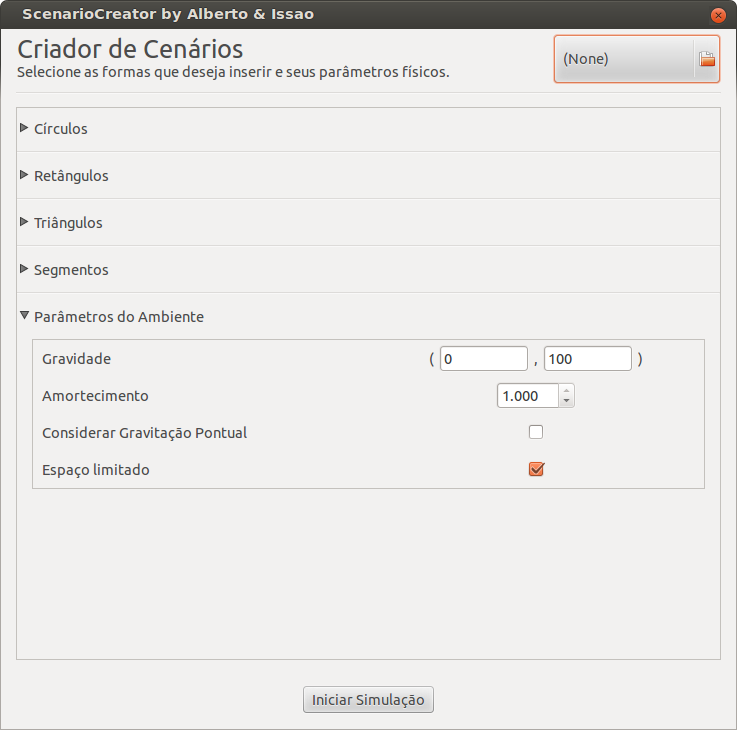
\includegraphics[scale=0.5]{telaInicial.png}
  \caption{Tela inicial do Physimulation}
\end{figure}

\newpage

\section{Discretização da simulação} \label{discretizacao}
\subsection{Tempo de simulação}
Tempo de simulação é o tempo utilizado para avançar a simulação de física por uma pequena quantidade de tempo.

\subsection{Tempo fixado}

\subsection{Tempo variável}

\newpage

\section{Colisões} \label{colisoes}
Uma das características das plataformas que suportam simulações físicas como o Chipmunk é a capacidade de detectar colisões entre os objetos. 
Para detectar colisões de forma eficiente essas plataformas utilizam um processo com duas fases: \textit{broad phase} e a \textit{narrow phase}.\\

A finalidade da \textit{broad phase} é evitar a realização de cálculos caros para corpos distantes um dos outros. Para
gerar os pares de objetos que devem passar pelo algoritmo de detecção de colisão, o Chipmunk suporta as seguintes estruturas de dados:
árvores AABB, \textit{1D sort and sweep} e o \textit{spatial hashing}. Na versão 5 do Chipmunk a estrutura de dados utilizada é o \textit{spatial hashing} enquanto na versão 6 são as árvores AABB. \\

\textit{Narrow phase} é a fase onde pares de objetos são verificados cuidadosamente em termos de colisão. O Chipmunk utiliza nesta fase o \textit{Separating Axis Theorem}, que suporta somente polígonos convexos. Devido a esse motivo, não é possível criar objetos côncavos no Chipmunk. \\

Nas próximas seções serão explicadas resumidamente os algoritmos de cada fase.

\subsection{\textit{Broad Phase} - Árvore AABB}

Para entender a árvore AABB, é preciso primeiro entender o que é AABB. AABB é um acrônimo para \textit{Axis Aligned Bounding Box}, ou seja, caixas delimitadoras de objetos 
em formas de retângulo alinhadas com os eixos x e y, como mostra a figura \ref{mariobb}:

\begin{figure}[!htbp]
  \centering
  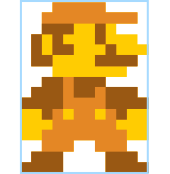
\includegraphics[scale=0.3]{mario_bb.png} 
  \caption{O retângulo azul representa uma caixa delimitadora do objeto}
  \label{mariobb}
\end{figure}

A árvore AABB é uma árvore binária que faz proveito da AABB para armazenar e consultar objetos no espaço 2D. O nó da árvore pode guardar o próprio objeto 
ou possuir dois nós filhos. Quando um nó guarda um objeto, a caixa delimitadora deste nó deve conter a caixa delimitadora do objeto. Se o nó possui nós filhos, 
sua caixa delimitadora deve conter as caixas delimitadoras dos nós filhos. 
Um ponto importante é que esta estrutura precisa de uma heurística para inserir os nós na árvore. No caso do Chipmunk existe uma heurística baseada na caixa 
delimitadora do objeto e também em relação à sua velocidade. Na figura \ref{aabb} mostramos um exemplo de uma árvore AABB de três objetos A, B e C: 

\begin{figure}[!htbp]
  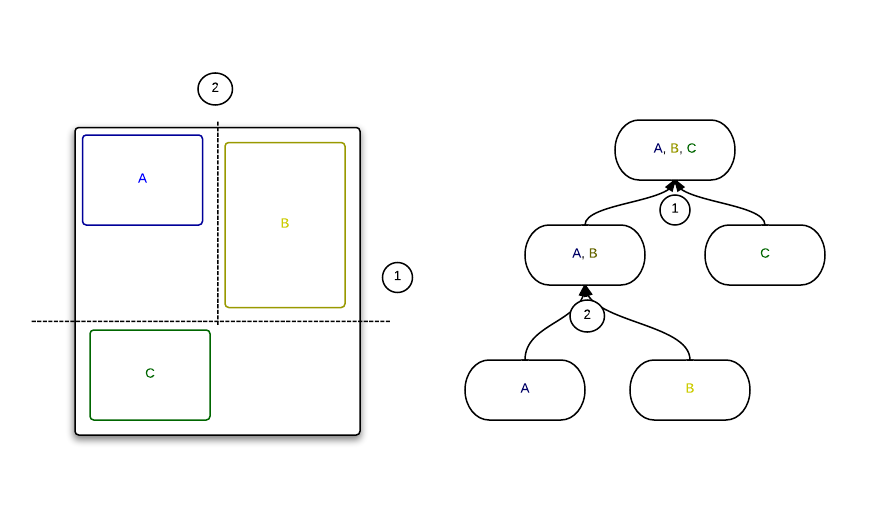
\includegraphics[scale=0.4]{AABBTree.png}
  \caption{Exemplo de uma árvore AABB}
  \label{aabb}
\end{figure}

A caixa delimitadora da raiz é o retângulo preto contendo os objetos A, B e C.
As duas novas caixas delimitadoras criadas pela linha indicado pelo número 1 são agora filhas da raiz. 
E finalmente a linha indicado pelo número 2 criam mais duas caixas delimitadoras separando os objetos A e B.\\

A figura \ref{aabbTree} mostra como são definidos os pares de objetos que passarão pela \textit{narrow phase}. Começando pela raiz, a caixa delimitadora do objeto D intersecta somente 
com a caixa delimitadora do nó esquerdo. Em seguida, a caixa delimitadora do objeto D intersecta somente com a caixa delimitadora da folha contendo o objeto A.
Então o par criado nessa busca é o par \{A, D\}.

\begin{figure}[H]
  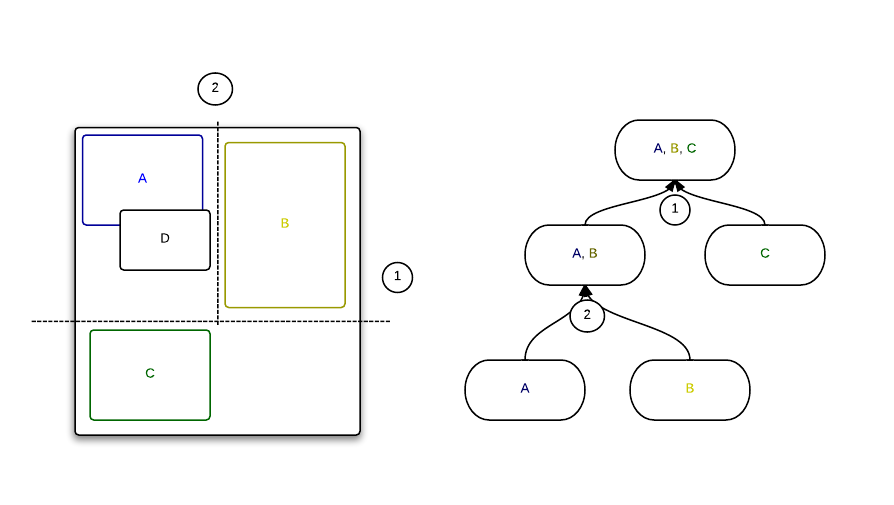
\includegraphics[scale=0.4]{AABBTree1.png}
  \caption{Exemplo de detecção de colisão. O objeto D é comparado somente com a folha contendo o objeto A.}
  \label{aabbTree}
\end{figure}

\subsection{\textit{Broad Phase} - 1D \textit{Sweep and Prune}}

A idéia deste algoritmo é varrer as caixas delimitadoras dos objetos criando assim os pares de objetos que deverão ser passados para a fase seguinte. \\

Seguindo o exemplo da figura \ref{sweep}, o algoritmo mantém uma lista de objetos que estão sendo varridos. Quando a varredura encontra o início do objeto, ela o inclui na lista. 
Quando a varredura encontra o final do objeto, ela o exclui da lista. No exemplo observamos que a lista [A, B, C] criam os pares \{A, B\}, \{A, C\} e \{B, C\} 
enquanto a lista [B, D] cria o par \{B, D\}. \\

\begin{figure}[!htbp]
  \centering
  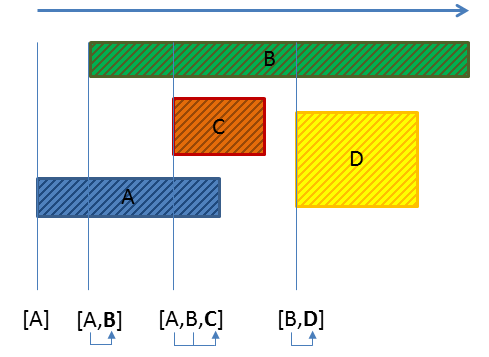
\includegraphics[scale=0.7]{sp.png}
  \caption{Exemplo de um algoritmo \textit{Sweep and Prune}}
  \label{sweep}
\end{figure}

Esse algoritmo, de acordo com a documentação do Chipmunk 6, pode ser muito eficiente em jogos voltados para dispositivos móveis se o seu mundo é muito comprido 
e plano como um jogo de corrida.

\subsection{\textit{Broad Phase} - Spatial Hashing}

\textit{Spatial hashing} é um processo onde o espaço de duas ou três dimensões é projetado em uma tabela \textit{hash} de uma dimensão. Para isso o Chipmunk divide o espaço em 
células do mesmo tamanho, onde cada célula é mapeada a uma entrada na tabela \textit{hash}. Um objeto sempre é mapeado nas células que ele está presente. Com esta estrutura 
  é fácil de criar os pares de objetos. Dado um objeto precisamos verificar quais as células que ele está presente e criar o par para cada objeto existente nas 
entradas da tabela destas células.\\

O tamanho das células é de suma importância para obter uma boa eficiência. Nas próximas figuras, as áreas cinzas representam as células. Quanto mais escuras, mais objetos estão mapeadas na célula. O ideal é que o tamanho das células não seja muito pequeno nem muito grande.\\

\begin{figure}[!htbp]
  \centering
  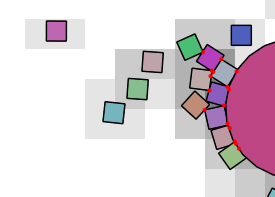
\includegraphics[scale=1]{hash_just_right.png}
  \caption{Cada célula contém poucos objetos. Estado ideal para \textit{Spatial hashing}}
\end{figure}

\begin{figure}[!htbp]
  \centering
  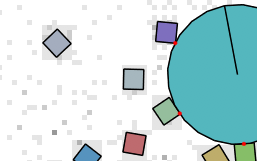
\includegraphics[scale=1]{hash_too_small.png}
  \caption{Cada objeto está mapeado em muitas células}
\end{figure}

\begin{figure}[!htbp]
  \centering
  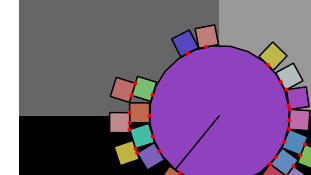
\includegraphics[scale=1]{hash_too_big.png}
  \caption{Cada célula contém muito objetos}
\end{figure}

Esta estrutura de dados é a mais indicada quando a simulação possui um conjunto grande de objetos e de mesmo tamanho.

\subsection{\textit{Narrow phase} - \textit{Separating Axis Theorem}}

No Chipmunk existe somente um algoritmo para detecção de colisão, baseado no \textit{Separating Axis Theorem}. A idéia do algoritmo é verificar se é possível desenhar um segmento 
de reta entre duas formas convexas. Se existe tal segmento, então não há colisão entre eles, caso contrário, as duas formas estão colidindo. No caso de formas
côncavas isso não é verdade. Devido a essa restrição do algoritmo o Chipmunk impõe que todo polígono seja convexo. \\

É um algoritmo rápido que elimina a necessidade de ter um código de detecção de colisão para cada tipo de forma. A figura \ref{narrow} ilustra a idéia do algoritmo.

\begin{figure}[!htbp]
  \centering
  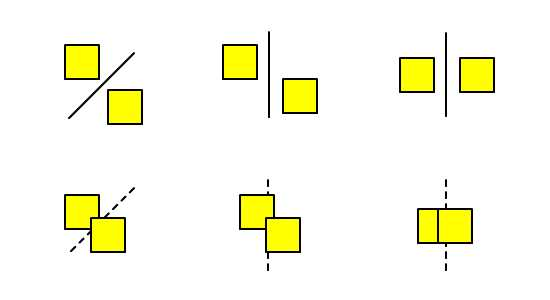
\includegraphics[scale=0.5]{SAT.jpg}
  \caption{Se existe uma linha que separa os polígonos convexos, então eles não estão colidindo.}
  \label{narrow}
\end{figure}

\newpage

\section{Atividades realizadas} \label{atividades}
Criamos algumas demonstrações básicas demonstrando a capacidade da plataforma Chipmunk e etc...

\subsection{Demonstrações}

falar sobre as demonstrações feitas.. Aqui tem que ficar bonito pq vamos colocar imagem

\subsection{Simulador}

falar sobre o que o simulador faz... 

\newpage

\section{Animações produzidas} \label{animacoes}
As animações de diferentes tipos de ambientes físicos foram nossos primeiros resultados obtidos. Após desenhar alguns cenários simples que ilustravam tópicos da disciplina de física, como descrito na seção \ref{atividades}, partimos para implementação. Nosso principal objetivo nesta etapa era compreender melhor o funcionamento do Chipmunk: seus conceitos, seus recursos e suas limitações. \\

Além disso, como tínhamos em mente implementar um criador de cenários, a medida que implementávamos estas demonstrações extraíamos todo código relevante para classes auxiliares que pudessem ser reutilizadas posteriormente. Atualmente, a classe {\tt physics.rb} contém grande parte deste código extraído. \\

\begin{lstlisting}[language=Ruby, caption=Trecho de código do physics.rb]
# @param [Hash] options : mapa com as opcoes de 
#           configuracao do objeto fisico.
def setup_trait(options = {})
  self.color =  options[:color] || Gosu::Color::WHITE
  self.zorder = options[:zorder] || 100
  self.factor = options[:factor] || options[:scale] 
    || $window.factor || 1.0
  @visible = true   unless options[:visible] == false

  if options[:static]
    @body = CP::StaticBody.new
  else
    @body = CP::Body.new(options[:mass], 
        options[:moment_inertia])
    @body.v = options[:v] if options[:v]  
    @body.w = options[:rotational_velocity] || 0
    @body.add_to_space($space)
  end
  (...)
end
\end{lstlisting}

\subsection{Descrição}

\begin{figure}[H]
	\centering
	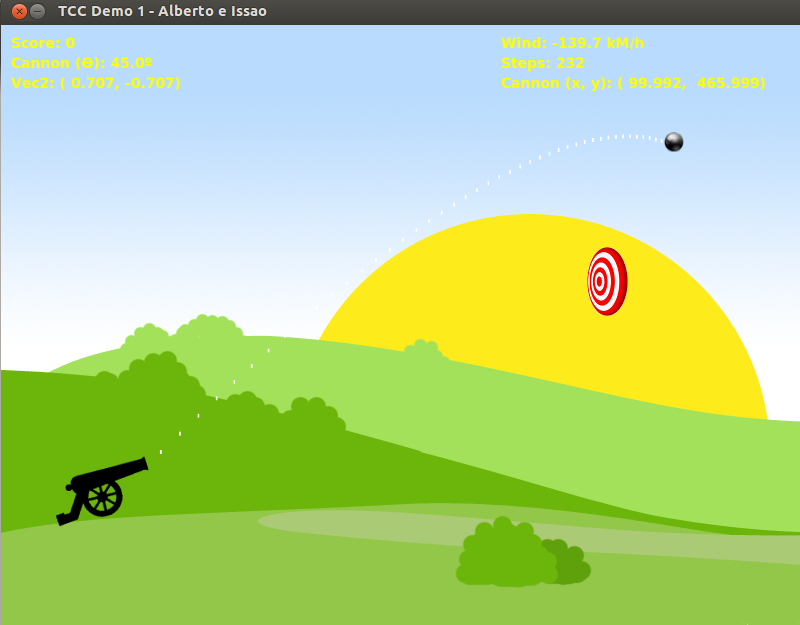
\includegraphics[scale=0.4]{images/cannonball.png}
	\caption{Cannonball}
	\hspace{0.5cm}
\end{figure}

\textit{Cannonball} foi nosso primeiro cenário físico. Baseado em jogos comuns de tiro ao alvo, como arco-e-flecha e catapultas, o objetivo é acertar uma bola de canhão em um alvo de posição escolhida aleatoriamente. O usuário pode modificar a angulação do canhão e atirar a bola pressionando a tecla de espaço. Há um vento de intensidade também calculada de forma aleatória, na direção horizontal e sentido contrário ao do trajeto da bola ao alvo. As informações relevantes ao usuário - ângulo do canhão, intensidade do vento, pontuação, entre outros - são exibidas no topo da janela. \\

Nossa intenção com este cenário era ilustrar o comportamento de lançamentos oblíquos e resistência do ar. \\

Posteriormente, utilizamos o código de \textit{Cannonball} na integração com exercício-programa \textit{Angry-Bixos}, descrita na seção \ref{ep}. \\

\newpage

\begin{figure}[H]
\centering
	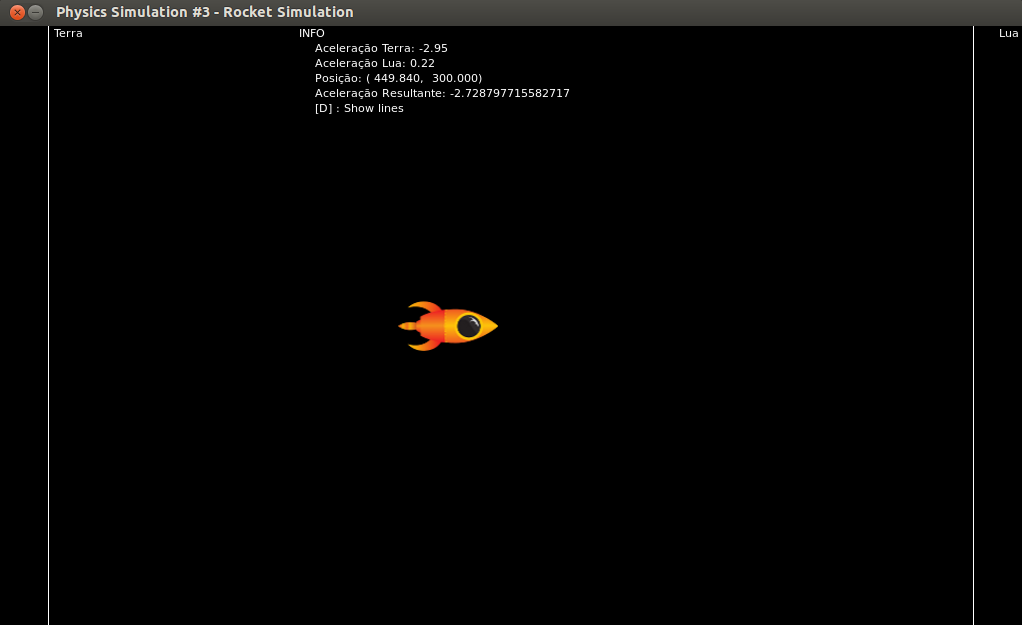
\includegraphics[scale=0.3]{images/rocket-simulation.png}
\end{figure}

\begin{figure}[H]
\centering
	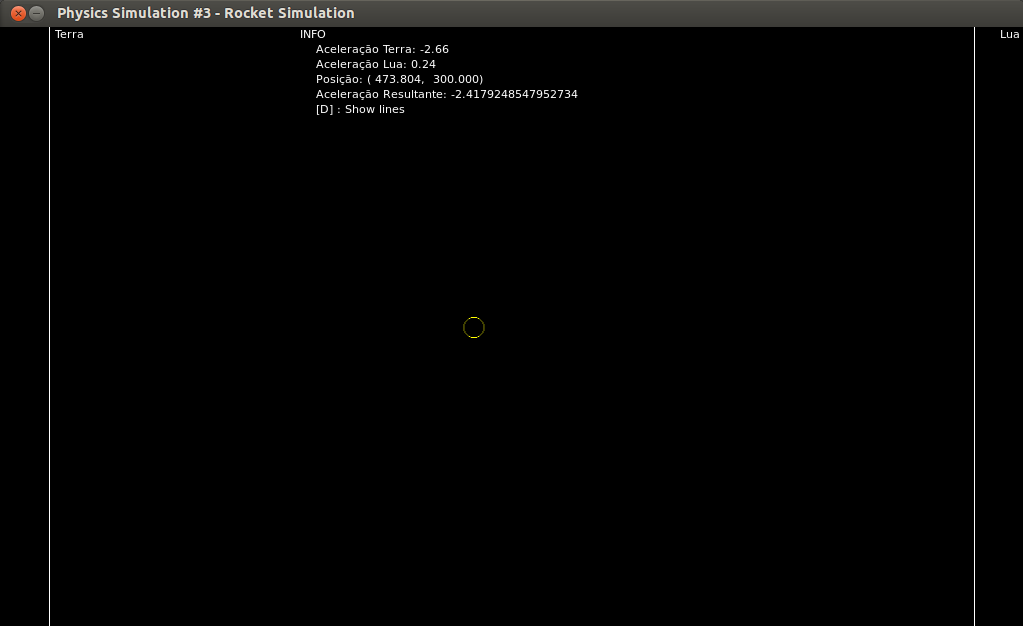
\includegraphics[scale=0.3]{images/rocket-simulationE.png}
	\caption{Rocket Simulation}
\end{figure}

A ação conjunta das gravidades da Terra e da Lua sobre um objeto é simulada em \textit{Rocket Simulation}. Controlando um foguete, o usuário pode movimentar-se com as setas do teclado entre os dois corpos, representados por retas nas extremidades esquerda e direita da tela. Por ter uma massa bem maior, a atração exercida pela Terra é maior em boa parte da tela, exceto em regiões bem próximas a Lua. \\

Por motivos de simulação, não reproduzimos os valores reais de massa de ambos os corpos, pois a região em que a Lua teria maior efeito sobre a nave seria ínfima e não proporcionaria ao usuário a experiência que gostaríamos. \\

\begin{figure}[H]
\centering
	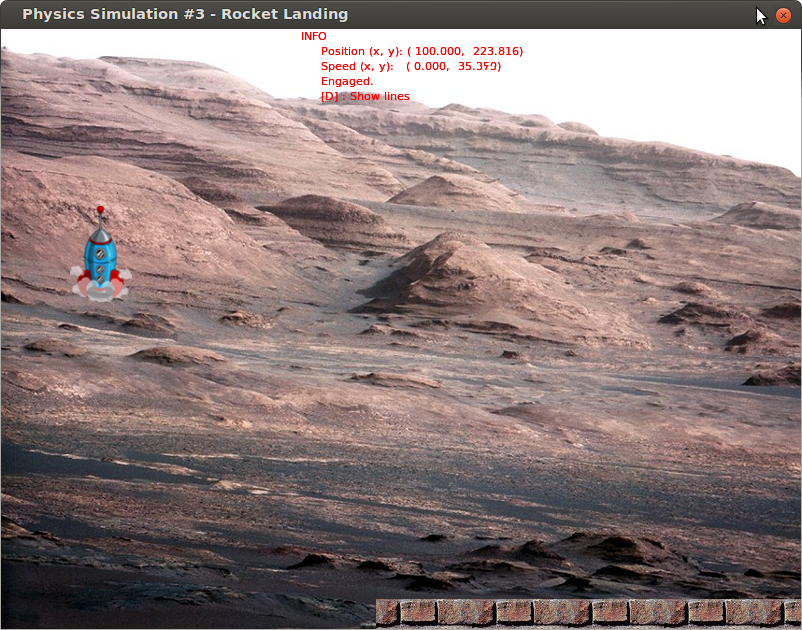
\includegraphics[scale=0.4]{images/lunarLanding.png}
\end{figure}
\begin{figure}[H]
\centering
	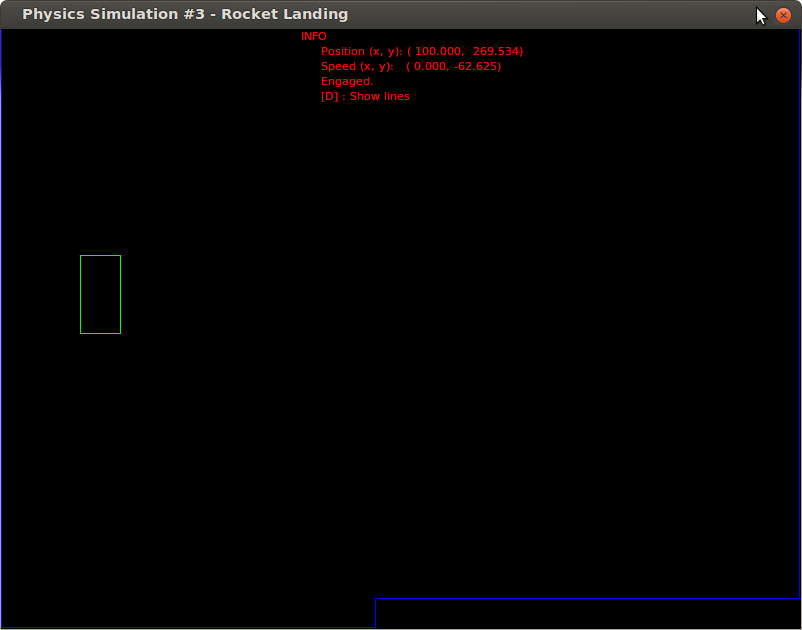
\includegraphics[scale=0.4]{images/lunarLandingE.png}
	\caption{Lunar Landing}
\end{figure}

Baseado no jogo \textit{Lander}, o objetivo é aterrisar um foguete em uma superfície plana com uma velocidade bem pequena. Se o usuário não conseguir diminuir adequadamente a velocidade antes de tocar a superfície, o foguete explode. Em caso de sucesso, ele pousa e uma mensagem de sucesso é exibida. As setas do teclado movimentam o foguete. \\

Com a implementação desta demonstração utilizamos em conjunto o código de detecção de colisão do \textit{Cannonball} com a manipulação de objetos de \textit{Rocket Simulation}. \\

Tanto neste e em outros cenários há a função ''Raio-X'' (tecla 'd'), que mostra ao usuário o esqueleto dos objetos do cenário. Em outras palavras, os \textit{shapes} que estão ativos no \textit{space} da simulação. Mais detalhes na seção \ref{plataforma}.

\begin{figure}[H]
\centering
  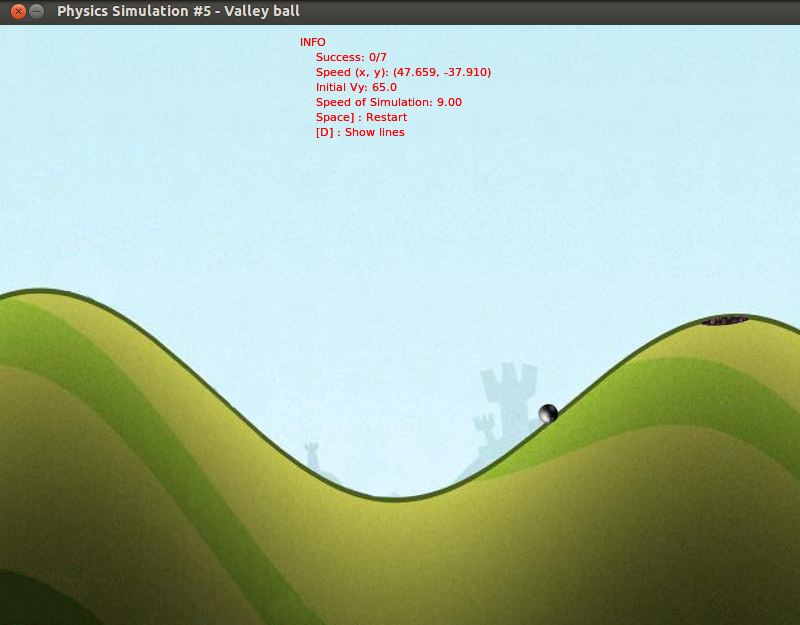
\includegraphics[scale=0.4]{images/valleyball.png}
\end{figure}
\begin{figure}[H]
\centering
  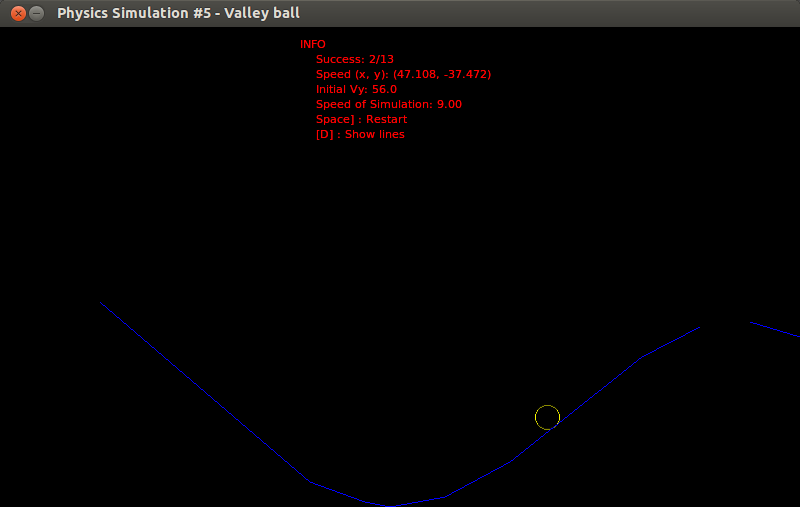
\includegraphics[scale=0.4]{images/valleyballE.png}
  \caption{Valleyball}
\end{figure}

Em \textit{Valleyball}, tentamos ilustrar o Princípio de Conservação da Energia Mecânica e a aplicação da força de atrito. Uma bola é lançada a uma certa altura do chão com velocidade vertical determinada aleatoriamente. Ela então desliza sobre um pequeno vale e dependendo da velocidade inicial ela pode: 1) voltar ao vale e perder velocidade até a situação de repouso; 2) cair em um buraco localizado próximo ao topo de uma montanha; ou 3) prosseguir seu movimento para fora do cenário. O que determina a situação resultante é a velocidade inicial da bola. A tecla de espaço reinicia a simulação com uma nova velocidade para a bola. \\

Nesta demonstração utilizamos pela primeira vez o controle de velocidade da simulação. Dentro de alguns limites, o usuário pode alterar o tamanho do passo da simulação (seção \ref{discretizacao}), tornando a animação mais rápida ou mais lenta. Isso é útil, por exemplo, para acelerar alguma etapa da simulação cujos resultados sejam previsíveis ou pouco interessantes. \\

\begin{figure}[H]
\centering
  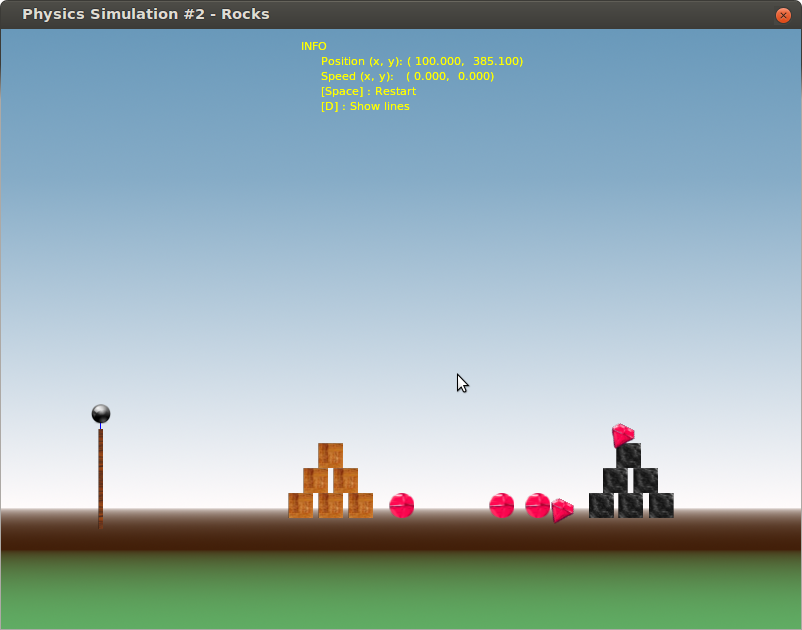
\includegraphics[scale=0.4]{images/rocks.png}
\end{figure}
\begin{figure}[H]
\centering
  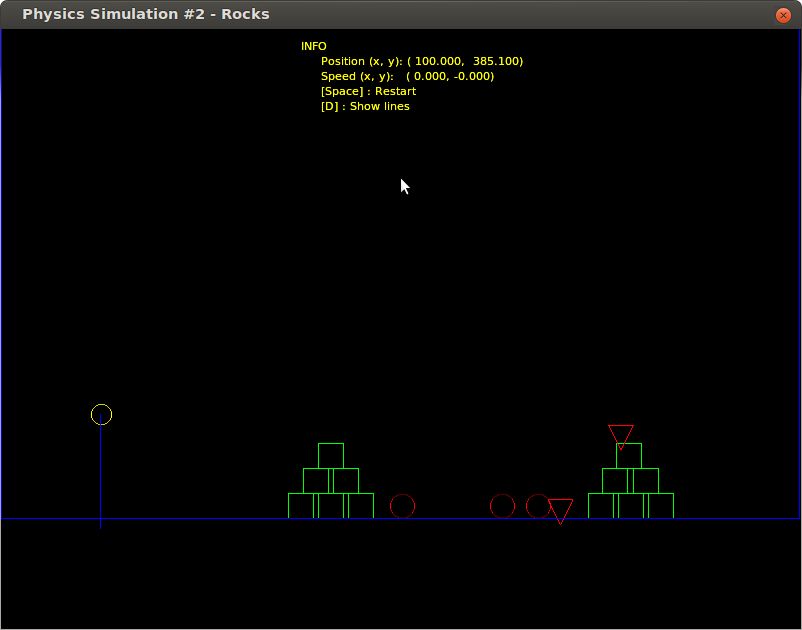
\includegraphics[scale=0.4]{images/rocksE.png}
  \caption{Rocks}
\end{figure}

\textit{Rocks} foi nosso último cenário de demonstração. Parecido com \textit{Cannonball}, o objetivo também é acertar alvos da tela - neste caso os objetos de cor vermelha. Porém é o usuário que determina a força que a bola será atirada, dependendo de quanto ele ''puxar'' a bola segurando e arrastando o \textit{mouse}, de modo semelhante ao comportamento de um estilingue. Com este cenário físico gostaríamos de simular um jogo que recentemente ficou bastante conhecido, o \textit{Angry Birds}. Além dos alvos, há cubos empilhados na tela, sendo estes de dois tipos: de pequena massa (cor de madeira) e de grande massa (cor de pedra). O resultado das colisões entre os objetos da tela variam de acordo com a massa do objeto. \\

Além de ser o único cenário de demonstração que possui interação com o \textit{mouse}, \textit{Rocks} consolidou nosso conhecimento das bibliotecas utilizadas e das modificações que precisávamos fazer para implementar o Physimulation. Em termos de física, a novidade deste cenário é a utilização de Energia Potencial Elástica no lançamento do objeto. 

\subsection{Visualização das animações}
Para visualizar as animações descritas nesta seção, o aluno deve executar o seguinte comando:

\begin{Verbatim}[fontsize=\footnotesize]
	$ cd <<DIR_PHYSIMULATION>>/Simulation
	$ ruby main.rb demos
\end{Verbatim}

onde {\tt\footnotesize DIR\_PHYSIMULATION} é o diretório em que o Physimulation foi instalado. Em seguida, deve escolher uma das animações listadas no programa e clicar em ''Iniciar''. Caso haja algum problema ao executar qualquer um dos comandos, verificar os passos da seção \ref{instalacao} (''\nameref{instalacao}'') foram seguidos corretamente.

\begin{figure}[H]
	\centering
	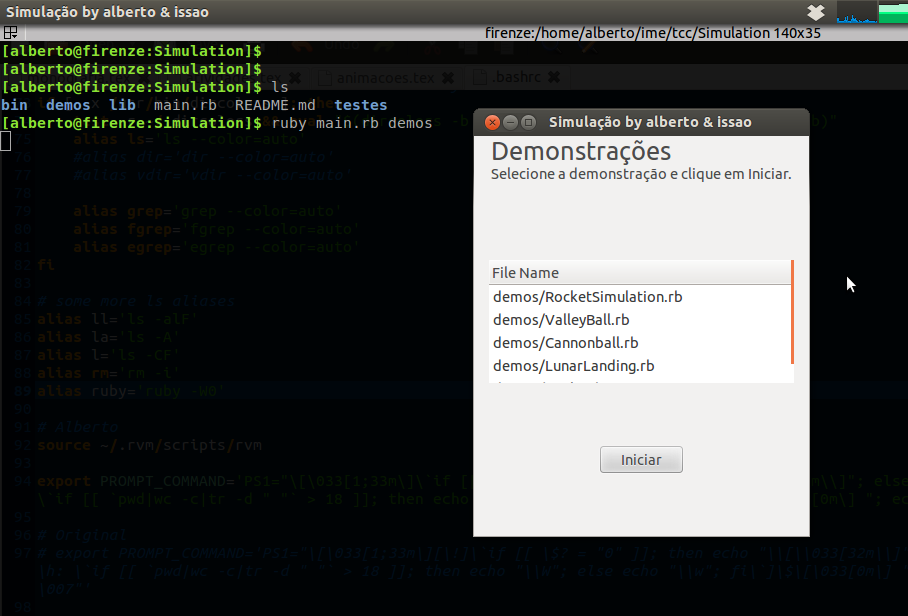
\includegraphics[scale=0.3]{images/demos-menu.png}
	\caption{Menu de demonstrações}
\end{figure}



\newpage

\section{Physimulation} \label{physimulation}
Descrição da interface de criação de cenários e alguns exemplos do que pode ser criado com ele.


\begin{figure}
	\centering
	\caption{Cenário 1}
	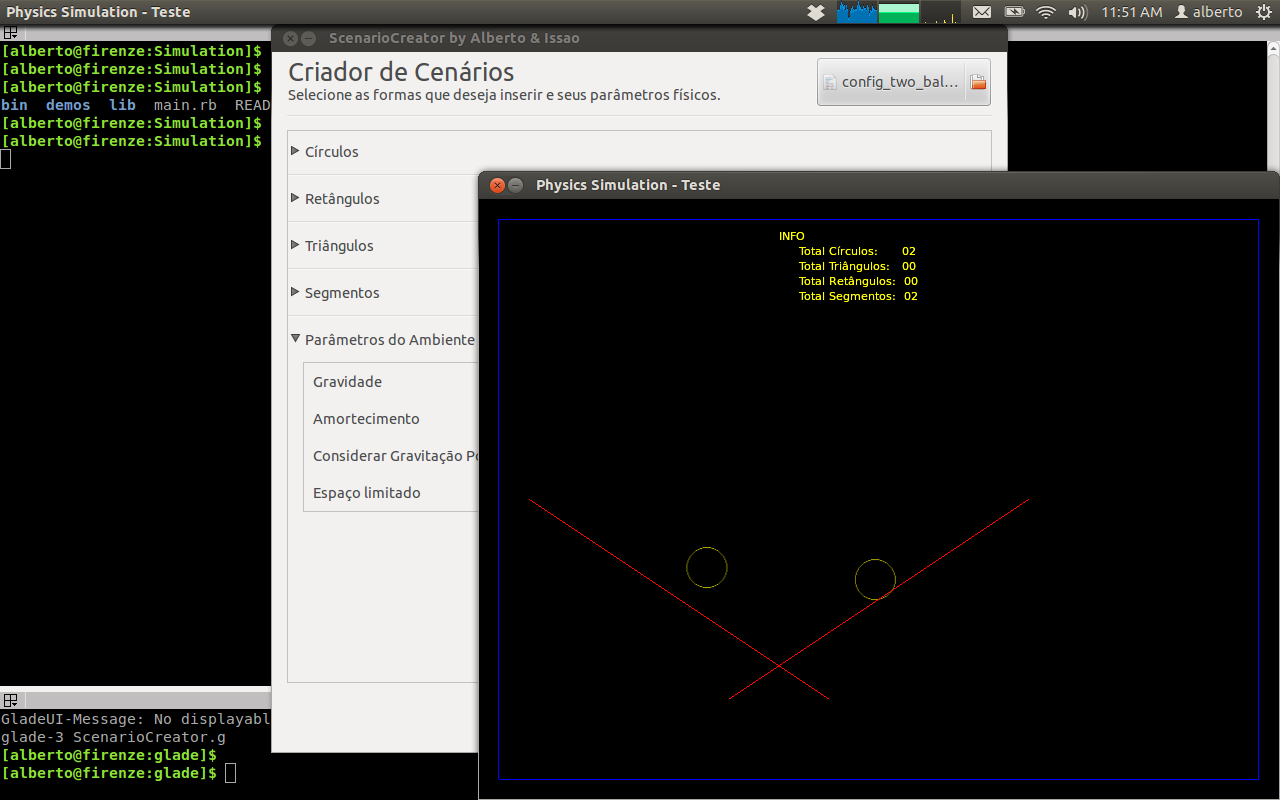
\includegraphics[scale=0.3]{images/cenario-two-balls.png}
	\hspace{0.5cm}
\end{figure}

  \begin{figure}
	\centering
	\caption{Cenario 2}
    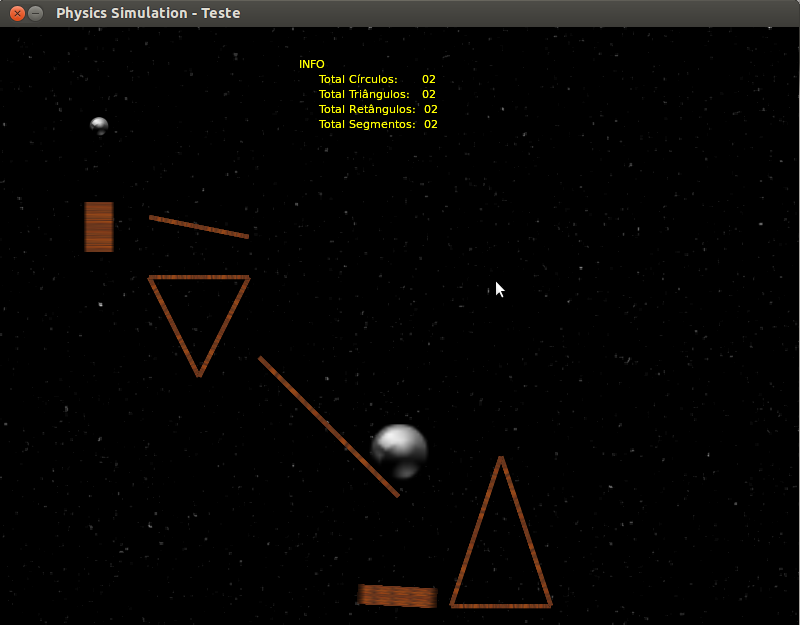
\includegraphics[scale=0.4]{images/cenario-todos.png}
    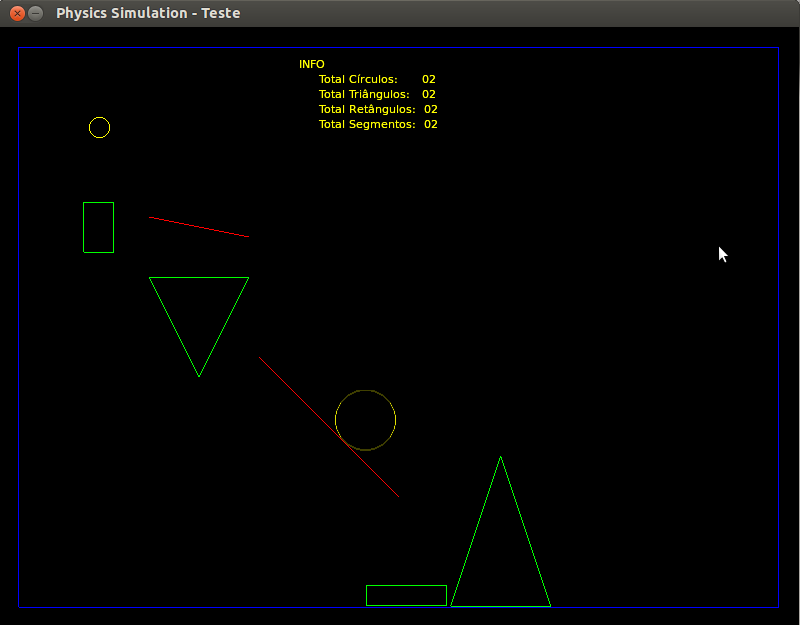
\includegraphics[scale=0.4]{images/cenario-todosE.png}
  \end{figure}

  \begin{figure}
	\centering
	\caption{Cenário Gravitacão 1}
    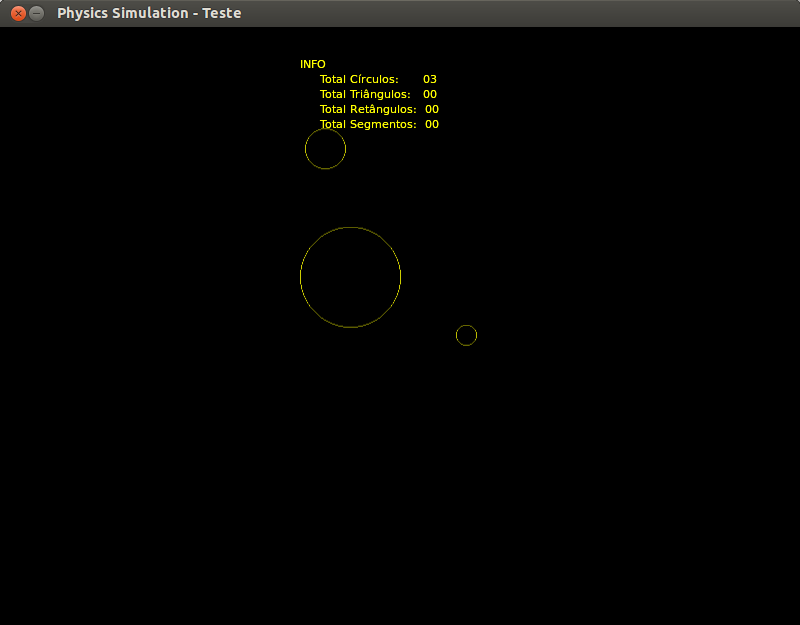
\includegraphics[scale=0.4]{images/cenario-gravitacao.png}
    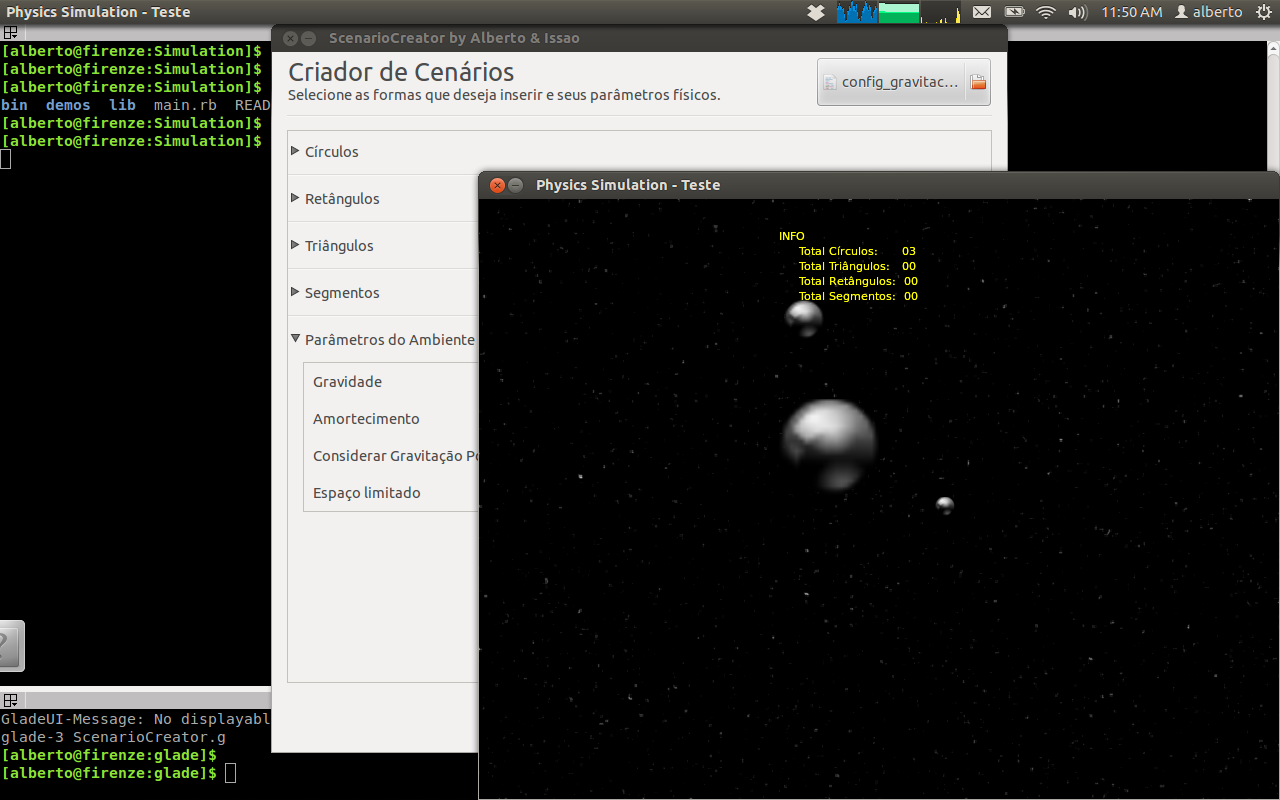
\includegraphics[scale=0.4]{images/cenario-gravitacao-2.png}
  \end{figure}

  \begin{figure}
	\centering
	\caption{Cenário Gravitacão 2}
    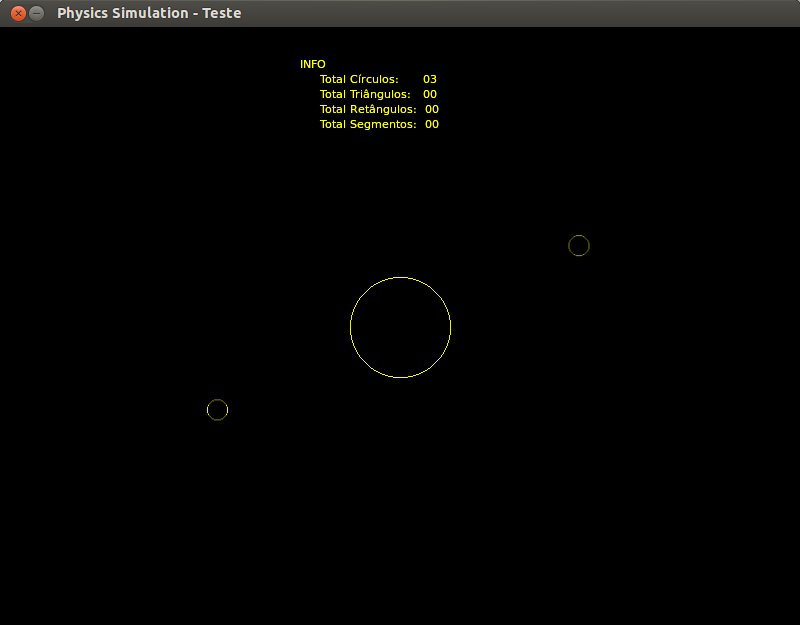
\includegraphics[scale=0.4]{images/cenario-gravitacao-3.png}
    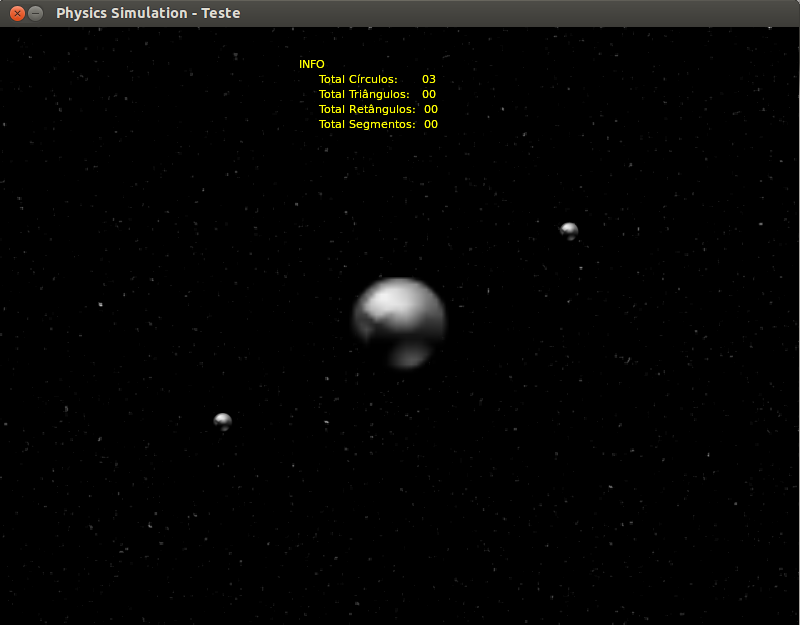
\includegraphics[scale=0.4]{images/cenario-gravitacao-4.png}
  \end{figure}


\newpage

\section{Introdução à computação com animações} \label{ep}
/*
Acrescentar algum exercício para o "aluno" fazer.
Pode ser

- um dos exercícios programas de MAC2166 que passei para
vocês, por exemplo o do "feito estilingue"
- o exercício seria "integrar" uma solução com a ferramenta de
vocês.

A ideia seria mostrar como um exercício programa de \\
MAC0110 ou MAC2166 pode ser transformado em algo visual (algo parecido com o que o Carlinhos falou)

*/


\newpage

\section{Conclusão} \label{comentarios}
\subsection{Trabalhos futuros}
\subsection{Conclusão}
\subsection{Desafios}


\newpage

\section{Instruções de instalação da plataforma} \label{instalacao}
\subsection{RVM - Ruby Version Manager}

RVM (Ruby Version Manager) é um gerenciador de versões de Ruby. 

\begin{enumerate}
\item Baixar e instalar o script do RVM.
\begin{verbatim}
$ curl -L https://get.rvm.io | bash -s stable
\end{verbatim}
\item Definir variáveis de ambiente.
\begin{verbatim}
$ source ~/.rvm/scripts/rvm
\end{verbatim}
\item Verificar se o RVM foi instalado corretamente.
\begin{verbatim}
$ type rvm | head -n 1
$ rvm is a function
\end{verbatim}
\end{enumerate}

\subsection{Ruby 1.9.3}

A versão 1.9.3 é utilizada pelo Physimulation.

\begin{enumerate}
\item Instalar o Ruby 1.9.3.
\begin{verbatim}
$ rvm install 1.9.3
\end{verbatim}
\item Verificar as versões instaladas do Ruby
\begin{verbatim}
$ rvm list
\end{verbatim}
\item Definir a versão do Ruby
\begin{verbatim}
$ rvm use 1.9.3
\end{verbatim}
\end{enumerate}

\subsection{Dependências do simulador}

Instalação das dependências do Physimulation.

\begin{enumerate}
\item Chipmunk
\begin{verbatim}
$ gem install chipmunk
\end{verbatim}
\item Gosu
\begin{verbatim}
$ gem install gosu
\end{verbatim}
\item Chingu
\begin{verbatim}
$ gem install chingu
\end{verbatim}
\item Visual Ruby
\begin{verbatim}
$ gem install visualruby
\end{verbatim}
\end{enumerate}


\newpage

\section{Apêndice} \label{apendice}
O texto a seguir foi extraído do site: \url{http://bcc.ime.usp.br}. \\

{\large \textbf{Material de Apoio ao BCC}} \\

A falta de contextualização das disciplinas básicas do BCC tem sido uma queixa recorrente do alunos nas reuniões entre alunos e professores, no Encontro do BCC de 2010 e também no processo de avaliação semestral que é realizado pelo orientador pedagógico orientador pedagógico da Escola Politécnica (POLI), Giuliano Salcas Olguin.\\

A fim de motivar os alunos e ilustrar a relação entre ciência da computação e as disciplinas básicas de álgebra, cálculo, estatística, probabilidade e física presentes no currículo do BCC a CoC sugeriu que fossem produzidos documentos ilustrando aplicação de cada uma dessas disciplinas em ciência da computação e vice-versa.  Esses documentos têm o objetivo de motivar os alunos do BCC:

\begin{enumerate}
\item ilustrando as relações entre as disciplinas básicas do curso e ciência da computação;
\item mostrando aos alunos quais das disciplinas mais avançadas do BCC que fazem uso dos conteúdos das disciplinas básicas;
\item fornecendo aos professores das disciplinas básicas do BCC exemplos de aplicações de suas especialidades em ciência da computação, que, eventualmente, podem ser mencionados em aulas ou ser temas de trabalhos.
\end{enumerate}

Esses documentos poderão também ser usados pelas disciplinas de Introdução à Ciência da Computação que são oferecidas pelo DCC para várias unidades da USP. Nestas disciplinas, frequentemente, os chamados exercícios programas ilustram aplicações de métodos computacionais na solução de problemas em genômica, física, economia, etc.
Por exemplo, na última edição da disciplina \begin{quote} MAC2166 Introdução à Ciência da Computação para Engenharia \end{quote}
podemos ver um exercício programa em que é simulada a "trajetória livre de retorno" de uma nave sob a ação gravitacional da Terra e da Lua em \url{http://www.ime.usp.br/~mac2166/ep3/}. Já um exercício programa com aplicação em genômica pode ser visto em \url{http://www.ime.usp.br/~mac2166/ep4/}.\\

Além de uma maior integração do curso este projeto pretende propor possíveis mudanças na grade curricular do BCC. Para isto pretendemos realizar uma pesquisa com o egresso do BCC e uma pesquisa das grades curriculares dos cursos de computação pelo mundo.

\newpage

\part{Parte subjetiva}
Nesta seção descreveremos a relação entre nosso projeto e a experiência adquirida no BCC.

(TODO pensei em fazer separado mas agora que escrevi tenho impressão que não vai mudar muita coisa)

\section{Alberto Ueda}
Entregar este projeto como trabalho de formatura e disponibilizar seu código para os alunos do BCC foram duas das experiências mais gratificantes que já tive. Isto pois acredito que tal conteúdo poderá ser utilizado pelas próximas turmas do BCC como incentivo ao aprendizado da matéria de física. Além disso, tanto alunos do próprio Instituto de Física quanto da Engenharia Politécnica também poderão se interessar pelo conteúdo: o primeiro grupo (FIS) pela animação de fenônemos físicos estudados e o segundo (Poli) tanto pela animação quanto pela simulação de tais fenônemos.

Mas, ao mesmo tempo, por ser um trabalho que levou meses, certas dificuldades foram encontradas pelo caminho. Tivemos que tomar decisões às vezes frustrantes, porém necessárias.

\subsection{Desafios e frustrações encontrados}
Inicialmente, nossa motivação era entregar um sistema que utilize recursos do Wii Remote (TODO ref TODO link da caneta) e que o professor pudesse utilizá-lo em sala de aula para realizar suas simulações e animações. Porém, chegamos a conclusão que esta tecnologia aumentaria consideravelmente o nível de complexidade de nosso trabalho e não tínhamos garantia de que utilizá-la acrescentaria da mesma forma ao resultado final. Assim descartamos esta possibilidade.

Como utilizamos algumas bibliotecas de terceiros em nosso projeto, tivemos que entender obrigatoriamente como eram feitas as principais chamadas de métodos destas bibliotecas, principalmente o Chipmunk e o Gosu. Um detalhe interessante que ocorreu no segundo mês de trabalho foi a necessidade de mudar o código da biblioteca (TOOD citar) e recompilá-la para que uma função simples de mensagem para o usuário funcionasse (TODO conferir método). Uma semana depois, utilizando uma versão mais nova da biblioteca, descobrimos que nossa alteração não era mais necessária, pois já havia sido feita pelos próprios programadores na mudança de versão.

Além disso, utilizamos um binding (TODO envoltório?) da versão original do Chipmunk. Isto trazia duas dificuldades para nós: 1) o código original (em C++) sempre estava com uma versão mais recente e provia (TODO conferir) mais métodos; e 2) nem sempre o que víamos na documentação oficial possuia correspondente em nosso binding. 
 
Por último, um desafio que tivemos foi encontrar um professor de física disponível para nos auxiliar na elaboração do protótipo do sistema. Ficamos muito felizes quando após algumas semanas o bacharel em física e aluno do BCC João Kerr veio a uma de nossas reuniões, a convite do professor Coelho.

\subsection{Disciplinas mais relevantes}

\begin{itemize}

\item MAC0110   Introdução à Computação : Embora já tivesse contato com programação no ensino técnico, foi nesta disciplina que passei a conhecer e utilizar boas práticas de programação. Além disso, estudei algoritmos famosos e interessantes (por exemplo os de ordenação) que estimularam-me para as disciplinas que viriam a seguir.

\item FAP0126 	Física I : É a grande motivação deste trabalho. Os conceitos aprendidos nesta disciplina estão por todo nosso código e nas simulações produzidas. Com o Physimulation, tentamos unir o que vimos nesta disciplina com a computação.
 
\item MAC0122 	Princípios de Desenvolvimento de Algoritmos : O maior contato com algoritmos, dos mais simples e elegantes aos mais complexos, foi fundamental para minha formação. Primeiro porque me desafiou em certos momentos - e consequentemente me deu coragem para analisar ou implementar futuros algoritmos - e em segundo lugar pois deu-me a confiança de que gostaria de seguir carreira em computação.
 
\item MAC0211 	Laboratório de Programação I : Esta disciplina foi interessante por dois motivos: pelo estímulo ao trabalho em equipe e por nos apresentar conceitos e ferramentas relacionadas a qualidade de software, como o Doxygen para documentação de código. Foi nesta disciplina que aprendi o que era um Makefile!

\item MAC0323 	Estruturas de Dados : Essencial para minha formação como cientista da computação. As estruturas aprendidas nesta disciplina - como listas ligadas e árvores - são muito comuns na programação, mesmo no mercado. Possuem vantagens e desvantagens entre si e o conhecimento de suas propriedades assim como os algoritmos adequados para manipulá-las foram muito importantes para mim.

\item MAC0420 	Introdução a Computação Gráfica : Outro forte motivador para nosso trabalho. Nesta disciplina tivemos como exercício-programa a simulação de um jogo de bilhar em três dimensões. Foi uma das experiências mais gratificantes do meu BCC, pois minha dupla e eu aplicamos física em um código simples em C com algumas bibliotecas gráficas e de repente tínhamos uma simulação razoável do que ocorre na vida real. Foi quando percebi que com poucos conceitos de física podíamos reproduzir muitos fenômenos naturais, como colisões e dissipação de energia. Percebi também o quanto estes resultados me motivavam a estudar mais, tanto física quanto computação.

\item FAP0137 	Física II : Os tópicos desta disciplina não foram o foco deste projeto, mas foram grandes motivadores para nosso trabalho. Assim como em Física I, houve pouca contextualização do que foi estudado com o curso de computação. No futuro, temas como relatividade restrita poderão se tornar bem mais simples de se entender por meio de animações criadas pelo próprio usuário, utilizando nosso simulador.
 
\item MAC0332 	Engenharia de Software : na área de computação, um dos conceitos mais recorrentes em qualquer projeto de longo prazo é ciclo de vida de um \textit{software}. Este era o tópico mais discutido na disciplina, tornando-a fundamental para o aluno de computação. Outro aspecto a destacar é a prática de trabalho em equipe.

\item MAC0338 	Análise de Algoritmos: difícil descrever em poucas linhas o quanto esta disciplina é importante para o aluno de computação. Além do desempenho ser uma preocupação constante e necessária a qualquer programador, o aprendizado nesta disciplina é uma das minhas bases sólidas como desenvolvedor. É uma das matérias que quero aprofundar meus conhecimentos durante o mestrado.

\item MAC0446 	Princípios de Interação Homem-computador : uma das disciplinas mais legais para o aluno que está preocupado com a usabilidade de seu sistema. Os conceitos aprendidos estão por todo o trabalho, assim como em outros projetos que participei ou fui responsável.

\end{itemize}
\subsection{Estudos futuros} 
Sem dúvida os tópicos de estudo mais importantes para a continuação deste trabalho são as disciplinas de Física I e II para o BCC. Quanto maior o conhecimento das leis e forças físicas presentes no mundo real, melhor serão as simulações e consequentemente as animações geradas.

Em segundo lugar, seria interessante uma análise de qual das alternativas a seguir tem uma melhor relação custo-benefício, visando a atualização do projeto com a versão mais nova do Chipmunk: A) migrar nosso projeto de Ruby para C++ e usar diretamente a versão original do Chipunk, sem bindings; ou B) atualizar o binding em Ruby adicionando os métodos e funcionalidades da versão mais recente em C++.

Por último, mas não menos importante, um estudo de paradigmas que proporcionem mais usabilidade ao usuário, substituindo o preenchimento obrigatório de formulários para criação de objetos físicos. Ex: \textit{drag-and-drop} do mouse para "arrastar" as formas geométricas, fornecendo os valores de massa, coeficientes de elasticidade e atrito \textit{a posteriori} (após o objeto já estar na tela).


\section{Rafael Miyagawa}

\newpage 

\bibliographystyle{ieeetr}
\bibliography{bibliografia}
\newpage
\end{document}

